\section{Event Detector}
\label{sec-detector}

\begin{figure}
\centering
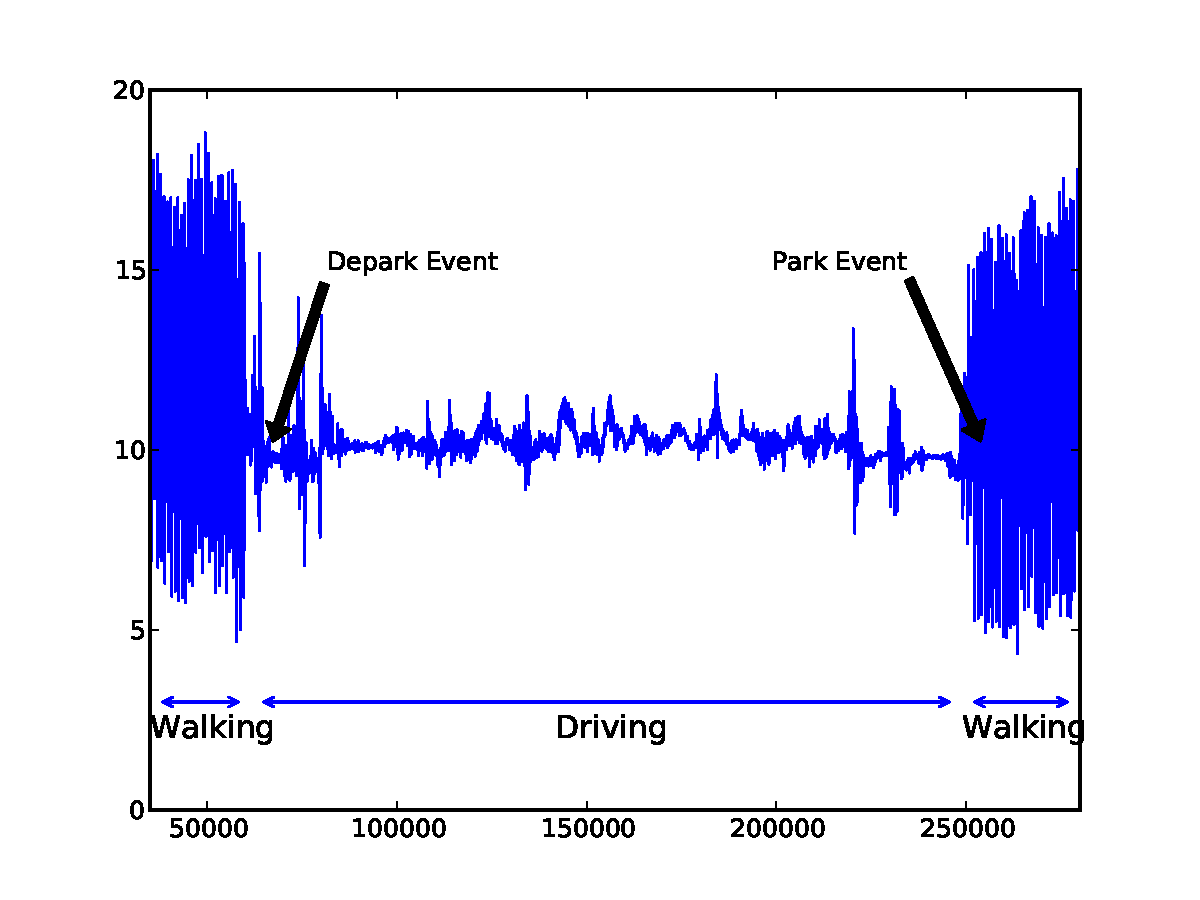
\includegraphics[width=\columnwidth]{./figures/Detection.pdf}

\caption{\textbf{Detection algorithm example.} The graph shows data collected
during our controlled experiment and shows a period of walking, followed by
driving, followed by a return to walking. Transitions between these states
indicate parking lot arrivals and departures.}

\label{fig-detectionexample}
\end{figure}

The inputs to PocketParker's availability estimation algorithm are arrival
and departure events generated by an activity detector running unattended in
each users pocket. While a great deal of previous research has explored
activity detection using sensors on mobile devices~\cite{FIXME}, we designed a
simple custom parking event detector tailored to the goals of PocketParker.
In addition to being designed and tuned to the specifics of our detection
problem, our event detector can also utilize the structure of our monitoring
problem to reduce false positives. In this section, we describe our event
detector and the portions of the PocketParker system that run on the
smartphone itself.

\subsection{Parking Events}
\label{subsec-goals}

PocketParker assumes that transitions between walking and driving that occur
in locations known to be parking lots constitute either arrival (driving to
walking) or departure (walking to driving) events. Thus, we must be able to
efficiently detect walking and driving activities, and detect transitions
fast enough to determine the location of the parking lot in which the event
took place. While all these states could be detected using
continuously-sampled GPS data, this would consume too much energy to be an
effective pocketsourcing solution. Instead, we rely on duty-cycled
accelerometer data to classify the user into one of three states: walking,
driving, or idle.

The application needs to determine the state of the user---whether walking,
driving or idle---with a test that is simple, quick and reasonably effective
for our goals.  We rely solely on accelerometer data for an initial
determination of state, as continuously cycled GPS sensing would consume too
much power. An accelerometer $\frac{1}{3}$ duty cycle, with 5~s sensing and
10~s idle periods, proved optimal. Five seconds was the minimum time
necessary to detect sensing activity accurately~\cite{FIXME}\XXXnote{GWA:
Anand: Need this reference if you can find it.}. We also wanted to obtain two
sensing periods within a short period of time for confirmation.

The initial test for user state relies on the standard deviation of sampled
accelerometer data within a sensing period. Our application first feeds
readings through a smoothing filter to suppress ambient sensor noise and
other low amplitude signals. A standard deviation of the processed signal of
less than $0.15\;\frac{m}{s^2}$ implies a user state of idle, a measurement
above $0.50\;\frac{m}{s^2}$ to that of walking, and values in between to
driving. The application stores a history of user states for future
reference. From this history, we define the user steady state to be whatever
state, if any, that constitutes a majority of the individual states observed
within the last nine periods.

We use user state, in turn, to deduce parking arrival events. The program
determines that a parking event has transpired upon fulfillment of several
conditions. The user steady state must be driving and the last two
individual states observed must be walking. Alternatively, if the steady
state is driving but only the last one state observed is walking, the program
imposes an additional constraint: the number of waveform peaks
$2\;\frac{m}{s^2}$ above the mean observed accelerometer value must exceed
a minimum threshhold corresponding to that produced by a slow human gait.
This test catches the large majority of parking events, where people park
their cars and immediately begin walking.

However, drivers occasionally sit in their cars for a period before leaving.
To detect this type of parking event, the program employs a second test.
Unfortunately, simply observing a state transition from driving to idle is
not, by itself, reliably determinative. While the walking and idle states
exhibit consistent well defined patterns, the driving state presents with
more fluctuation. The steady state of driving often contains individual idle
state periods. Rather, the program concludes that a driver has parked only
when the user steady state transcends from driving to idle to walking within
a three-minute period.

When the program concludes that a user has parked, it turns on GPS detection
long enough to determine the walking velocity and bearing of the user. It
then calculates backwards to estimate the location where the user started
walking---i.e., the parking spot. The mobile application reports the
occurrence and location of the newly detected parking event to the server via
HTTP. The server verifies the reported event against a pre-compiled list of
known parking lot locations before recording the event. This final step
eliminates events that are either incorrect---a user apparently parking in
a field---or unwanted---a user genuninely parking but in a loading area rather
than in a parking lot.

Occasionally, a user upon parking will walk for too brief a period before
entering a building for the program to obtain a location from GPS. On our
campus, this is an uncommon occurrence in practice, as there are few parking
spots close enough to buildings to produce this behavior. A reliable watermark
for this rarity is a steady driving state coupled with a most recent
individual walking state and a null GPS reading. In this situation, we employ
alternative Android location providers such as WiFi to determine user locale.

While walking, users may change their bearing. If this occurs before the
first GPS fix, the app may not be able to calculate the original location of
the parking spot. An apparent remedy to this would be to use compass data to
detect changes in bearing. This would work if the relative orientation of the
phone viz-a-viz the user were also detectable. In practice though, when not
in use mobile phones are typically oriented randomly by users, particularly
when placed in pockets and backpacks. Sticking solely with GPS data has thus
proven better. Going forward, maintaining a history of user pedestrian
history should further minimization of bearing inaccuracies.

A final potential issue with detecting a parking event is that of handling a
driving period too short to for the program to detect that a user is driving
in the first place. This situation would occur when a user simply moved his
car to a new parking spot in an adjacent row. This is not a worrisome problem,
as it does not stem from rational user behavior.

We employ user state transitions to detect parking departure events in a
manner similar to that used to detect parking arrivals. Our program
tentatively detects a departure event when the user steady state is walking
but the two most recent individual states are driving. The constraint of two
consecutive driving states rather than one proved necessary to minimize
spurious detection of driving due to the relatively variable nature of
accelerometer-determined driving sense data.

Before reporting a departure event, our mobile program employs GPS sensing to
confirm a driving state. In theory, it is unnecessary to turn on the GPS
system, as we have already previously determined the parking spot location
when the user first parked. Rather, we have still found doing so aids
ferreting out remaining falsely detected driving states. A null GPS reading
implies that a user is indoors, and that our initial inference of a driving
state was misplaced.

The application reports confirmed parking departure events to the HTTP
server. As with arrival events, departure event locations are matched against
a known list of lot locations to filter false reporting.

\subsection{Filtering False Positives}
\label{subsec-false}

Incorrect parking arrival and departure events stem in part from the
underlying issue of false detection of the individual driving state. The
relatively variable accelerometer data patterns produced when driving---and
that are often counterfeited by intermittent walking---complicate reliable
detection of this state. Happily, a sizable bulk of these false positives
consists of the case where users eventually simply walk indoors. Mandating
that a vaild GPS reading accompanies a preliminary driving state
determination allieviates this subset, albeit at the price of additional
power consumed.

False detection of both arrival and departure events could be further
minimized by using more accurate but computationally intense algorithms that
implement machine learning or Fourier transforms. We have deliberately shied
away from such an approach however, as the inherent nature of our application
dictates that the bulk of testing and filtering takes place on an
energy-constrained mobile platform. A more promising approach to reducing
false detection and a subject for further research would be to employ
additional location services.
